%%In this part we will look at statistics as well as to look at different formulas and application. furthermore we will look at the state of the art programs that apply these statistical calculation such as excel and mathcad ? 

%%skal være en omkring normal statestik og ikke hardcore gym/uni niveau 
statistics is the science of finding significant trends and deviations from a given set of data either grouped or non-grouped. In this part we will look at different statistical concept such as middle value, spread, variant and graphs derivations. 

%basic terms 
a basic concept of statistic is the observation. An observation is simply the set of samples we want to calculate on in our statistical investigation. The total number of samples in a set is typically described as \(n\). With our set, we can calculate the percentages the frequency of a give sample is of a set. We calculate the percentile frequency by the formulae: 
 
\[ p_i = \frac{f_i} {n} \]
 
where \(p_i\) is the percentage of sample \(i\) and \(f_i\) is the frequency of sample \(i\). The accumulated percentile frequency is simply the sum of all the percentile frequencies going from smallest to biggest sample.

\[ (acc.\ p)_i = p_1 + p_2 + ... + p_{i-1} + p_i = \sum\limits_{a=1}^i p_a \]

What we have been working with until now is called non-grouped observations. That is the set is just raw numbers without any manipulations done. non-grouped observation is preferred when we have a small number of samples in a set, and the samples appear multiple times, any. We can group the non-grouped observation but the data would not be nearly as detailed as it would otherwise. When we, on the other hand have a lot of samples, or the samples predominately have the frequency 1, we would get more details out of the data if we grouped the set in intervals. With grouped observation we introduce two new terms: interval frequency and interval percentile frequency, the former is the number of times that interval occurs, the latter is the percentile occurrences of the interval. 
An non-grouped observation is easiest to visualise in a bar chart whereas a grouped observation is easiest visualised in a histogram. A bar chart is where the name of the samples is out on the x-axis, and the frequency is out on the y-axis, the namesake of the chart will then visually represent the frequency of a given sample. A histogram are very similar to the bar chart but can only be done on a grouped observation. sometimes there will not be a y-axis on a histogram but a legend in the corner where an area is shown and a number in the area which shows the percentage that area represents, the total area of the bars/pillars of the histogram should be 100\%  

to give an example of the above:

    In a class we are interested in finding the age and the high of the pupils. the result where as follows:
    
    \begin{table}[H]
        \centering
        \begin{tabular}{r l c c c c c c c c c }
            Age =& \{14 & 14 & 14 & 15 & 15 & 15 & 16 & 16 & 16 & 13\} \\
            Height =& \{165 & 166 & 170 & 150 & 167 & 180 & 172 & 155 & 177 & 181\} \\
        \end{tabular}
    \end{table}
    
    the total number of samples in each set is n = 10
    we keep the age set as non-grouped and group the height set with interval length of five:
        
        \-\hspace{2cm} height = \{[150], [155], [165, 166, 167, 170], [172], [177], [180, 181]\}
        
    the frequency of 14 is 3, and to calculate the percentile frequency of 14 we use the formulae
    
        \[p_{14} = \frac{f_{14}} {n}\]
        
    which is 
    
        \[30\% = \frac{3} {10}\]
        
    the interval frequency of [165,170] is 4 and we calculate the percentile interval frequency in the same way as the percentile frequency 
        
        \[40\% = \frac{4} {10}\]
    
    to find the accumulated percentile frequency we simply add all the percentile frequencies together, this will often be 99,9 or 100,1 this discrepancy is caused by round errors.
    
    a bar diagram of the age set would look like:
    
    \begin{figure}[ht]
    \centering
    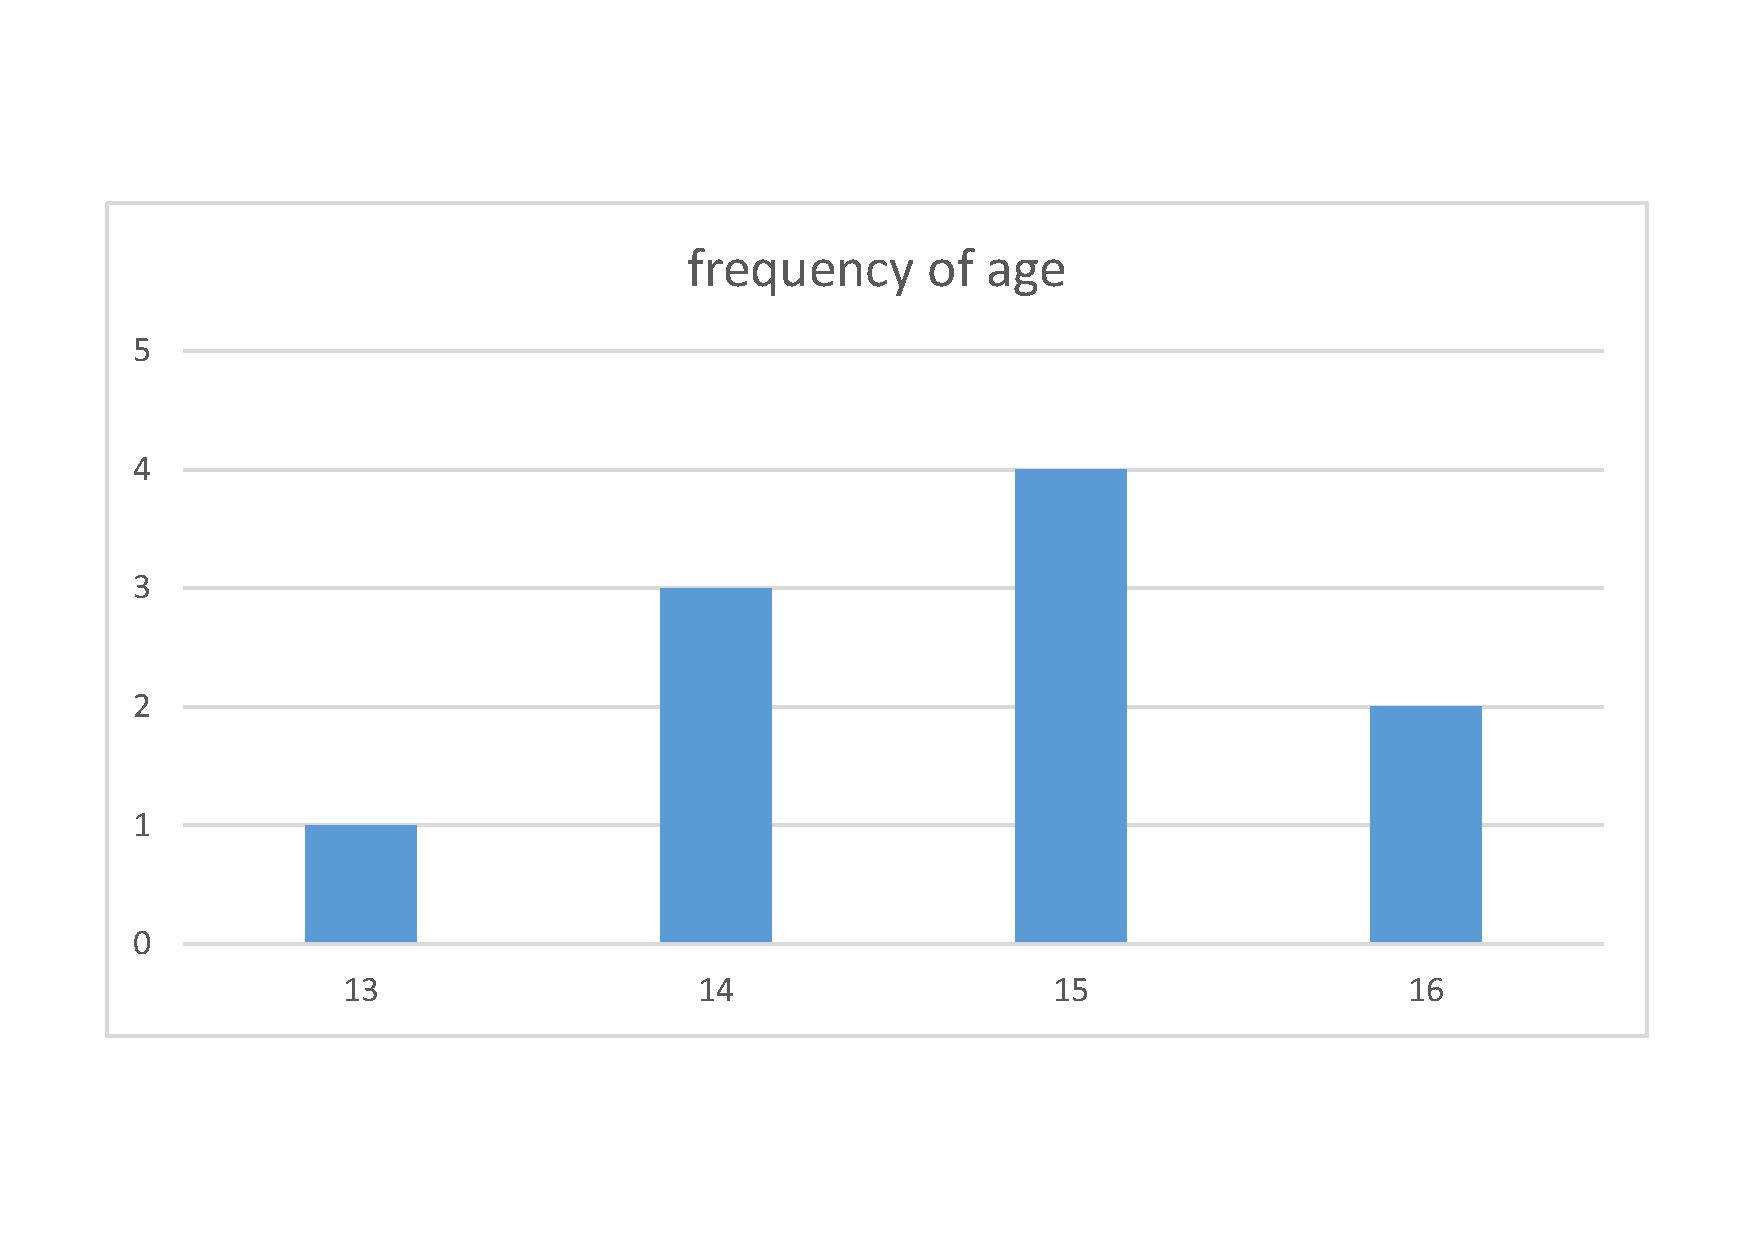
\includegraphics [width=12cm]{images/Frequency_age.pdf}
    \caption{}
    \label{fig:frequency_age}
    \end{figure}
    
    a histogram of the height set with a y-axis would look like: 
    
    \begin{figure}[ht]
    \centering
    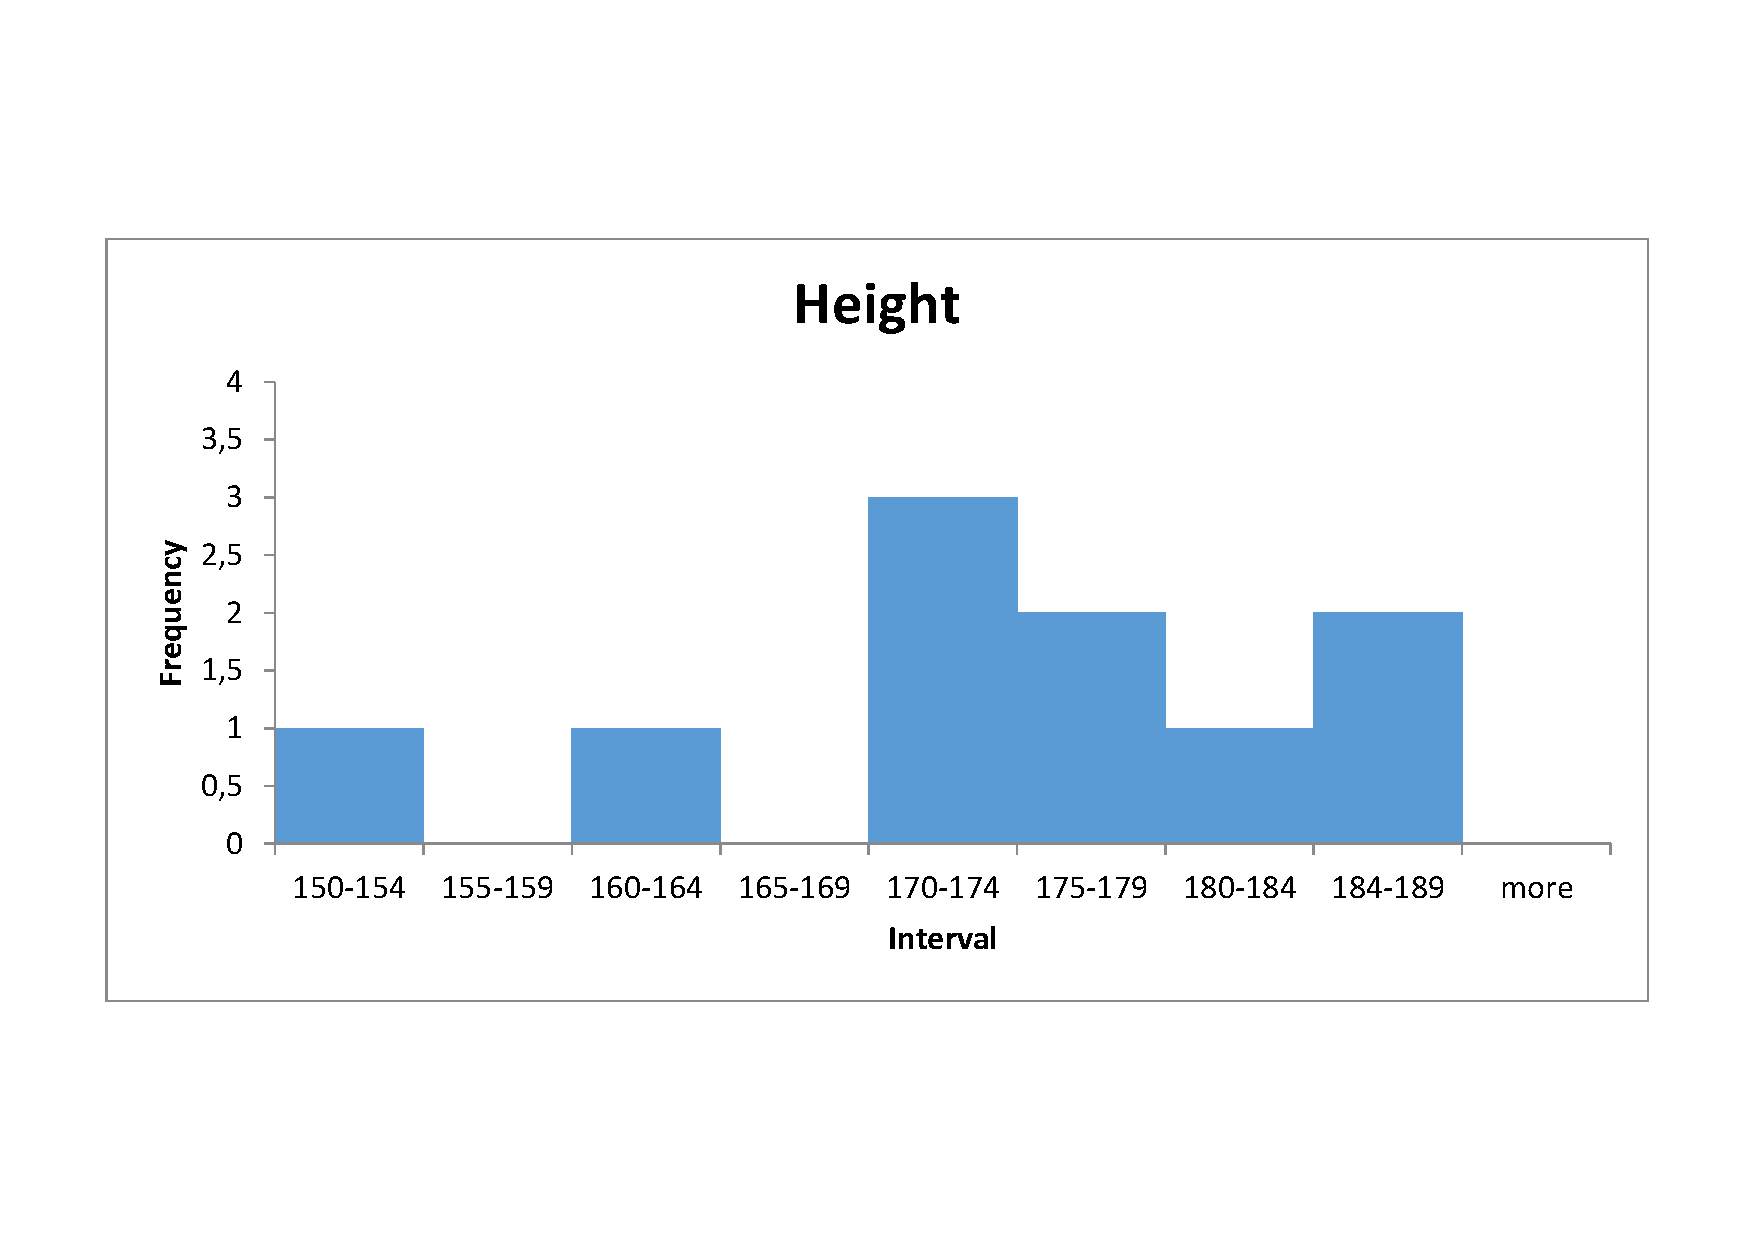
\includegraphics [width=12cm]{images/Height.pdf}
    \caption{}
    \label{fig:Height}
    \end{figure}
    
The Median, is the sample that separates the upper values from the lower value in a data set. in a 7 sample data set with rising values the median is quite simply the 4Th sample. If there is an equal number of sample the median is calculated by taking the sum of the two numbers in the middle and divide it by 2. 

The mean, or the average, on the other hand are quite simply the average of the sum of all the samples in a set and denotes by \(\overline{x}\). to calculate the mean we simply multiply the frequency with its sample and take the sum of the multiplications, we then divide the sum with the total number of samples. 
this gives us the formulae: 

\[ \overline{x} = \frac{1}{n} * \sum\limits_{a=1}^i f_a * x_a = \frac{f_1 * x_1 + f_2 * x_2 +...+ f_i * x_i}{n} \]    
    
where \(x_i\) is the iTh sample.

we can also calculate it from the frequency with the formulae: 

\[ \overline{x} = \sum\limits_{a=1}^i p_a * x_a = p_1 * x_1 + p_2 * x_2 +...+ p_i * x_i\]

We can't do the same with a grouped observation. This is because we can't multiply the value of the sample with the frequency because the samples are the whole interval and not just one value. 
we need to first find a median-value for the interval from the start \(a\) to the end \(b\) we find this by taking the sum of \(a\) and \(b\) and divide with 2, or in other words: 

\[ m = \frac{a+b}{2}\]

to then find the mean we simple change out value \(x\) with the median-value \(m\)

now that we have found out how we calculate the mean we can find out the variance and spread. the variance we calculate by finding the distance between the set and the mean value square it and find the average of it, or in other words

\[Var(x) = \frac{1}{n} * \sum\limits_{a=1}^i f_a *( \]


